\documentclass{article}
\usepackage[utf8]{inputenc}
\usepackage[spanish]{babel}
\usepackage{listings}
\usepackage{graphicx}
\graphicspath{ {images/} }
\usepackage{cite}

\begin{document}

\begin{titlepage}
    \begin{center}
        \vspace*{1cm}
            
        \Huge
        \textbf{Nociones de la memoria del computador}
            
        \vspace{0.5cm}
        \LARGE
        Proyecto de investigación
            
        \vspace{1.5cm}
            
        \textbf{Juan Andres Urbiñez Gómez}
            
        \vfill
            
        \vspace{0.8cm}
            
        \Large
        Departamento de Ingeniería Electrónica y Telecomunicaciones\\
        Universidad de Antioquia\\
        Medellín\\
        Septiembre de 2020
            
    \end{center}
\end{titlepage}

\tableofcontents
\newpage
\section{Definición de memoria del computador}
La memoria del computador se podría definir como dispositivo donde se almacena información temporalmente para luego ser llevada a procesador, estos usualmente su capacidad y velocidad son opuestamente proporcionales, es decir, a mayor capacidad, menor velocidad y viceversa.
\section{Tipos de memoria conocidas anterior a investigación} 
Antes de hacer esta investigación solo conocía muy pocos tipos de memoria siendo, RAM, cache, y el disco duro.

\subsection{Memoria RAM}
Random Acess Memory o por sus iniciales <<RAM>> (Figura \ref{fig:ram}) en pocas palabras es la que toma parte de información del disco duro de algún proceso activo en el computador, y almacenarlo temporalmente para luego procesarlo. Al ser memoria temporal, al apagar el computador la información en la RAM  desaparece.

\begin{figure}[h]
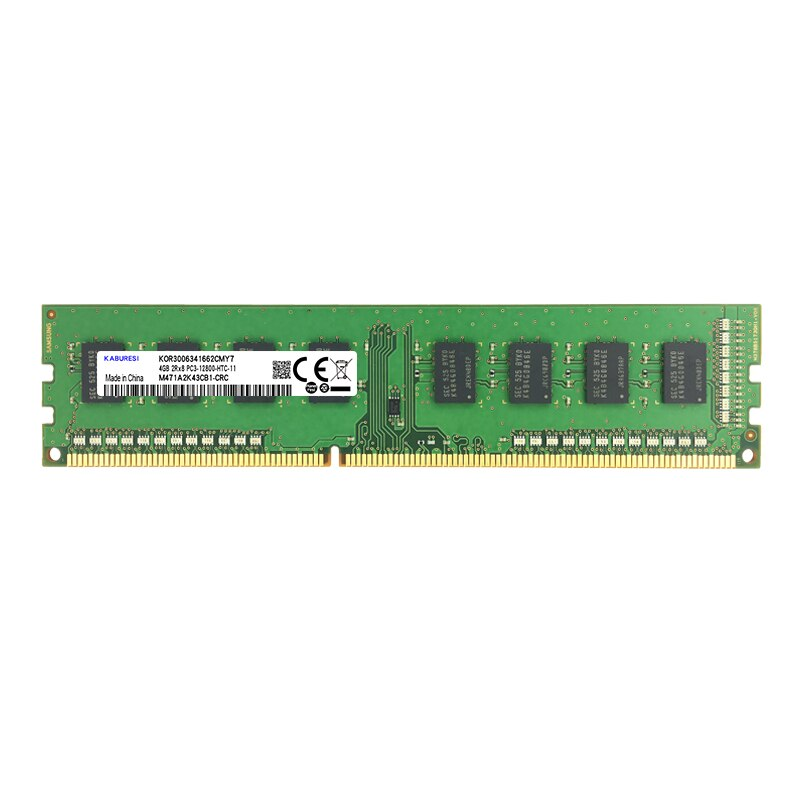
\includegraphics[width=4cm]{Images/Ram.jpg}
\centering
\caption{Memoria RAM}
\label{fig:ram}
\end{figure}

\subsection{Memoria cache}
La memoria cache a diferencia de la <<RAM>> esta muy cerca de la CPU (tanto que usualmente las CPU vienen con la memoria cache) para que la información requerida por la CPU llegue manera inmediata esta hay 3 tipos de memoria cache L1, L2, Y L3, donde L1 es la mas cercana a la CPU y L3 la mas alejada, en cuanto a capacidad $L1 < L2 < L3$.



\subsection{Disco duro}
El disco duro (Figura \ref{fig:discoduro}) es donde se almacena toda la información del computador que a diferencia de la RAM, en este no se pierde al apagarlo.

\begin{figure}[h]
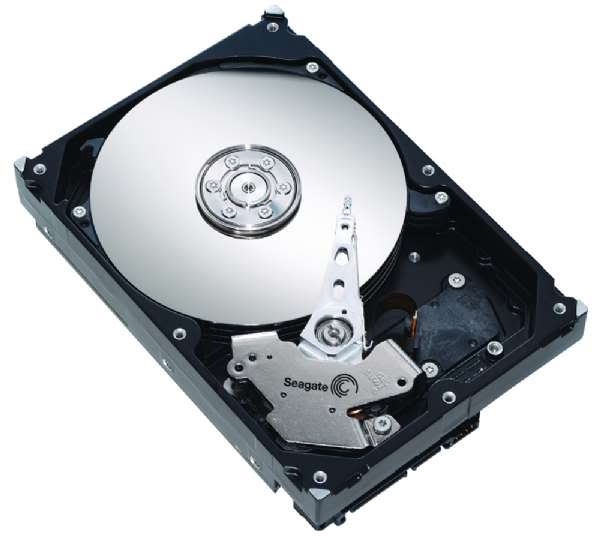
\includegraphics[width=4cm]{Images/discoduro.jpg}
\centering
\caption{Disco duro}
\label{fig:discoduro}
\end{figure}

\section{Gestión de memoria en el computador}

\section{Rapidez de memoria ¿Que la causa?}

\section{Conclusión} \label{conclulsion}

\bibliographystyle{IEEEtran}
\bibliography{references}

\end{document}

